\documentclass[11pt]{article}

\usepackage[utf8]{inputenc}
\usepackage{color}
\usepackage{graphicx}
\usepackage{geometry}
\usepackage{ltablex}
\usepackage{hyperref}
\hypersetup{
    colorlinks,
    citecolor=black,
    filecolor=black,
    linkcolor=black,
    urlcolor=black
}

\renewcommand{\contentsname}{Inhaltsverzeichnis}

\begin{document}

\begin{titlepage}
	\begin{center}
		\vspace*{1cm}

		\Huge
		\textbf{Tourney}\\
		Spezifikation

		\vspace{0.5cm}
		\LARGE
		Softwarepraktikum\\
		\Large
		Wintersemester 2014/2015

		\vspace{1.5cm}

		\large
		\textbf{Jonas Auer (2860992)\\
				 Fabian Biester (2859084)\\
				 Jan Tagscherer (2893134)}

		\vfill

		
\includegraphics[width=0.4\textwidth]{Logo.png}

		\vspace{1.5cm}

		\Large
		Universität Stuttgart\\
		14.11.2014
	\end{center}
\end{titlepage}

\newpage

\tableofcontents
\newpage

\section{Einleitung}

\subsection{Zweck der Spezifikation}

Dieses Dokument dient dem Zweck, sowohl funktionale als auch qualitative Anforderungen überprüfbar, vollständig und systematisch festzuhalten. Damit ermöglicht es dem Kunden und den Betreuern sicherzustellen, dass die richtige Funktionalität auf korrekte Art und Weise umgesetzt wird. Um dies zu gewährleisten muss die Spezifikation als wichtiger Leitfaden während der Entwicklung und für alle weiteren erstellten Artefakte beachtet werden. Zudem müssen sowohl die Spezifikation als auch weitere betreffende Dokumente aktuell gehalten werden.

\subsection{Leserkreis}

Der Leserkreis dieses Dokuments setzt sich aus den folgenden Personengruppen zusammen:
\begin{itemize}
	\item Das Projektteam:
	\begin{itemize}
		\item Die Entwickler
		\item Die Gutachter während des Reviews
		\item Die Betreuer
	\end{itemize}
	\item Der Auftraggeber
	\item Mit der Wartung und Weiterentwicklung betraute Software-Entwickler
\end{itemize}

\subsection{Einsatzbereich und Ziele}

In diesem Projekt wird die Organisationssoftware \textbf{Tourney} umgesetzt. Diese setzt sich zum Ziel, die Planung und Durchführung von Spielturnieren deutlich zu vereinfachen.

Zuvor fand die Organisation dieser Turniere weitestgehend manuell statt, indem Anmeldungen und Ergebnisse auf Papier oder per Tabellenkalkulation aufgezeichnet wurden. Dies führte zu starken Verzögerungen und deutlich mehr Arbeit im Rahmen eines solchen Turniers.

Mit dem Einsatz von \textbf{Tourney} entfällt unnötiger Mehraufwand, indem Events und deren Turniere modular verwaltet werden. Dazu gehören sowohl das Führen von Datenbe-ständen wie Voranmeldungen, Anmeldungen und Turnierergebnissen als auch das automatische Auswerten von Spielresultaten anhand bearbeitbarer Spielregeln und die Verteilung einiger Daten über Turnierordner oder weitere administrative Arbeitsplätze mit anschließendem Zusammenfügen.

Die Software wird im Rahmen des Softwarepraktikums im Wintersemester 2014/2015 an der Universität Stuttgart und unter Auftrag des Heidelberger Spieleverlags entwickelt.

\subsection{Fachbegriffe und Abkürzungen}

Relevante Fachbegriffe und deren Abkürzungen sind in der Spezifikation \textit{kursiv} markiert und werden im Begriffslexikon geklärt, das diesem Dokument anhängt.

\subsection{Übersicht und Aufbau des Dokuments}

Um die zu entwickelnde Software vollständig zu spezifizieren wird das Dokument in die nachfolgenden Kapitel gegliedert:
\begin{itemize}
	\item[] \textbf{Kapitel 2} gibt einen groben Überblick über grundlegende Funktionen, über die die Software verfügen soll, in welchem Umfeld und von welchen Nutzern sie eingesetzt wird und welche Einschränkungen und Annahmen bei der Entwicklung eingegangen werden.
	\item[] \textbf{Kapitel 3} beschreibt die konkreten Anforderungen, die vom Auftraggeber an die Software gestellt werden. Dabei werden zwischen funktionalen und qualitativen Anforderungen unterschieden.
	\item[] \textbf{Kapitel 4} charakterisiert Nutzer und für die Software relevante Personengruppen.
	\item[] \textbf{Kapitel 5} enthält Skizzen als Prototyp der geplanten Benutzeroberfläche.
	\item[] \textbf{Kapitel 6} umfasst grundlegende Anwendungsfälle, die bei der Benutzung der Software auftreten können und die die Interaktion der Nutzer mit dem Programm umreißen.
	\item[] \textbf{Kapitel 7} umschließt ein Begriffslexikon, in dem alle wichtigen Fachbegriffe und Abkürzungen geklärt werden.
\end{itemize}

\section{Allgemeine Beschreibung}

\subsection{Einbettung}

Bisher wurden keine Softwarelösungen zur Organisation von Spielturnieren eingesetzt. Deshalb muss \textbf{Tourney} in keine bestehenden Systeme eingebettet werden.

\subsection{Einschränkungen bei der Entwicklung}

Aufgrund der geforderten Plattformunabhängigkeit wird die Software in der Programmiersprache Java entwickelt. Dabei können die Versionen 1.7 oder 1.8 verwendet werden.

Zusätzlich können die folgenden Bibliotheken verwendet werden:
\begin{itemize}
	\item Grafische Benutzeroberfläche mit \textbf{Swing} oder \textbf{JavaFX}
	\item Datenbankeinbindung durch \textbf{H2} in Verbindung mit \textbf{JDBC}
	\item Erstellen von PDF-Dokumenten mit \textbf{iText}
\end{itemize}

\subsection{Grundlegende Produktfunktionen}

Die Software soll grundsätzlich die folgende Funktionalität haben, die in Kapitel 3 ausführ-licher beschrieben wird:
\begin{itemize}
	\item Modulare Erstellung von Regelmodulen für konkrete Spielturniere
	\item Planung von Events und Festlegen von stattfindenden Turnieren
	\item Verwalten von Spielerlisten in Hinsicht auf Voranmeldung, Anmeldung bei Anwesenheit und Bezahlstatus
	\item Durchführung und Auswertung von Turnieren anhand spezifizierten Regeln und An-zeigen von Paarungen über eine Projektion
	\item Zusammenführen und Ausgeben der Turnierresultate am Administrationsrechner
	\item Verteilen von relevanten Datenbanken zum kollaborativen Arbeiten während Anmeldungen und an die Turnierordner mit jeweils anschließendem Zusammenfügen der Daten
\end{itemize}

\subsection{Benutzermerkmale}

Die Nutzer von \textbf{Tourney} sollten zur erfolgreichen Bedienung keine besonderen Kenntnisse besitzen müssen. Insbesondere sollte die Oberfläche so selbsterklärend sein, dass dies auch ohne Lesen des Handbuchs möglich ist. Die Benutzer besitzen hierbei für gewöhnlich zwar Fachkenntnis in Bezug auf die Spielturniere, allerdings sollte kein besonderes technisches Wissen vorausgesetzt werden. Vielmehr sollte die Software so intuitiv zu bedienen sein, dass für keinen Nutzer ein Hindernis entsteht.

Desweiteren kann nicht davon ausgegangen werden, dass sowohl die Arbeitsplätze von Administratoren als auch Turnierordnern ausreichend abgesichert sind. Deshalb sollten relevante Daten über Passwörter zusätzlich gesichert sein.

Zuletzt sollte versehentlichem Datenverlust durch eine übergreifende Rückgängig-Funktion vorgebeugt werden.

\subsection{Annahmen und Abhängigkeiten}

Um die Software erfolgreich entwickeln und betreiben zu können muss von den folgenden externen Einflussfaktoren ausgegangen werden:
\begin{itemize}
	\item Die erforderliche Hardware zur Ausführung des Programms und Massenspeichergeräte zur Datenübertragung müssen zur Laufzeit bereitgestellt werden.
	\item Die Turnierregeln dürfen sich nicht so stark ändern, dass die modulare Regelerstellung nicht mehr relevant ist. In diesem Fall kann eine korrekte Ergebnisauswertung nicht mehr garantiert werden.
	\item Aufgrund des engen zeitlichen Rahmens dürfen in späten Projektphasen keine fundamentalen Änderungen an den Anforderungen mehr erfolgen.
\end{itemize}

\section{Spezifische Anforderungen}

\subsection{Funktionale Anforderungen}

\subsubsection{Mengengerüst}

\subsubsection{Leistungsanforderungen}

\subsubsection{Externe Schnittstellen}

\subsubsection{...}

\subsection{Qualitätsanforderungen}

\subsubsection{Bedienbarkeit}

Zur Bedienung von \textbf{Tourney} sowohl als Administrator als auch als Turnierordner werden keine weitreichenden technischen Kenntnisse gefordert. Entsprechend sollte die Software sich gegenüber Nutzereingaben möglichst defensiv verhalten und auf fehlerhafte Eingaben verständlich aufmerksam machen. Weitere nutzerseitige Fehler werden durch eine Rückgängig-Funktion abgefangen.

Das Bedienkonzept zielt auf eine intuitive Interaktion ab, die auch ohne das Lesen eines Handbuchs möglich ist. Dazu müssen alle Module und zeitliche Abläufe konsistent und übersichtlich gekapselt werden. Alle Elemente der Oberfläche sollten eindeutig bezeichnet sein ohne dass dies überladen wirkt.

Kritische Aktionen wie das Löschen von Daten müssen durch Dialoge bestätigt werden.

\subsubsection{Erweiterbarkeit}

Um eine hohe Änderbarkeit und Erweiterbarkeit zu gewährleisten werden große Teile der Software modular gestaltet, etwa die Abtrennung von Administrator- und Turniermodul oder die Verwendung änderbarer Regelmodulen.

Auch interne Komponenten der Software werden in abgeschlossene Einheiten mit hohem Zusammenhalt und geringer Kopplung gegliedert. Desweiteren sollen Redundanzen so gut wie möglich vermieden werden.

Eine umfangreiche Dokumentation auch durch Kommentierung im Code und die konsistente Anwendung der \href{http://www.oracle.com/technetwork/java/codeconvtoc-136057.html}{\textbf{Code Conventions for the Java\texttrademark\ Programming Language}} stellen eine hohe Lesbarkeit zur späteren Anpassung sicher.

\subsubsection{Sicherheit}

Da keine Schnittstellen mit einem externen Netzwerk bestehen und die Daten über Massenspeichergeräte übertragen werden, müssen diese nicht in besonderem Maße verschlüsselt werden. Allerdings sollte die unrechtmäßige Manipulation der Datensätze verhindert werden, indem diese durch Passwörter sowohl auf Seiten der Administratoren als auch der Turnierordner gesichert werden. Zudem können diese Personen ihre jeweiligen Arbeits-plätze bei vorübergehender Abwesenheit sperren.

\subsubsection{Zuverlässigkeit}

Die Software übernimmt in der Turnier- und Eventorganisation eine zentrale Rolle. Kommt es während dem Betrieb zu einem längerfristigen Ausfall oder Datenverlust, kann das geplante Event nicht ohne erheblichen Mehraufwand und erneutes Erfassen der erforderlichen Daten durchgeführt werden. Zu derartigen Problemen sollte es also keinesfalls kommen.

Ein kurzfristiger Ausfall ist in diesem Sinne also nicht besonders kritisch, wenn er nur zu geringen Verzögerungen führt, sollte aber in Anbetracht der Nutzerfreundlichkeit bestmöglich vermieden werden.

\subsubsection{Portabilität}

Da die Software mit der Programmiersprache Java und unter Verzicht auf native Schnittstellen entwickelt wird ist eine umfassende Portabilität mit einer Vielzahl von Plattformen gegeben.

\section{Benutzerprofile}

\subsection{Administrator}

Der Administrator hat übergreifenden Zugriff über die erstellten Datensätze. Er kann Events erstellen, Turniere hinzufügen und verwaltet Spieleranmeldungen. Diese Daten kann er teilweise auch im Nachhinein bei Bedarf abändern. Zudem kann der Administrator Auszüge aus den erstellten Datensätzen an weitere Benutzer weitergeben, einerseits um Anmeldungen an mehreren Arbeitsplätzen vorzunehmen, andererseits um Spielerlisten und Turniereigenschaften an die Turnierordner zu übergeben. Nach diesen Vorgängen werden die erhobenen Daten wieder beim Administrator zusammengefügt.

Beim Administrator handelt es sich um den Organisator des Events. Auch bei dieser Person werden keine besonderen technischen Kenntnisse vorausgesetzt.

\subsection{Turnierordner}

Turnierordner haben die Aufgabe, tatsächlich anwesende Spieler bei den jeweiligen einzelnen Turnieren zu erfassen und dann die Spiele durchzuführen. Dabei werden von der Software Paarungen vorgeschlagen und nach dem Spielende die Resultate eingetragen. Diese Daten lassen sich auch später noch manuell abändern. Zudem kann der Turnierordner Spieler disqualifizieren. Für diese Vorgänge werden die vom Administrator übertragenen Daten verwendet.

Ein Turnierordner ist zumeist eine Person mit guten Kenntnissen der Spielregeln und sollte die Verantwortung über die Datensätze übernehmen können.

\subsection{Spieler}

Die Spieler sind die größte Nutzergruppe. Sie führen keine direkte Interaktion mit der Software durch, sondern sollen sich über Ausgaben und Projektionen über Paarungen und Spielstände informieren können. Dazu müssen diese leicht verständlich und weithin lesbar sein.

\section{Benutzeroberfläche}

\subsection{...}

\section{Anwendungsfälle}

\subsection{Übersicht über die Anwendungsfälle}

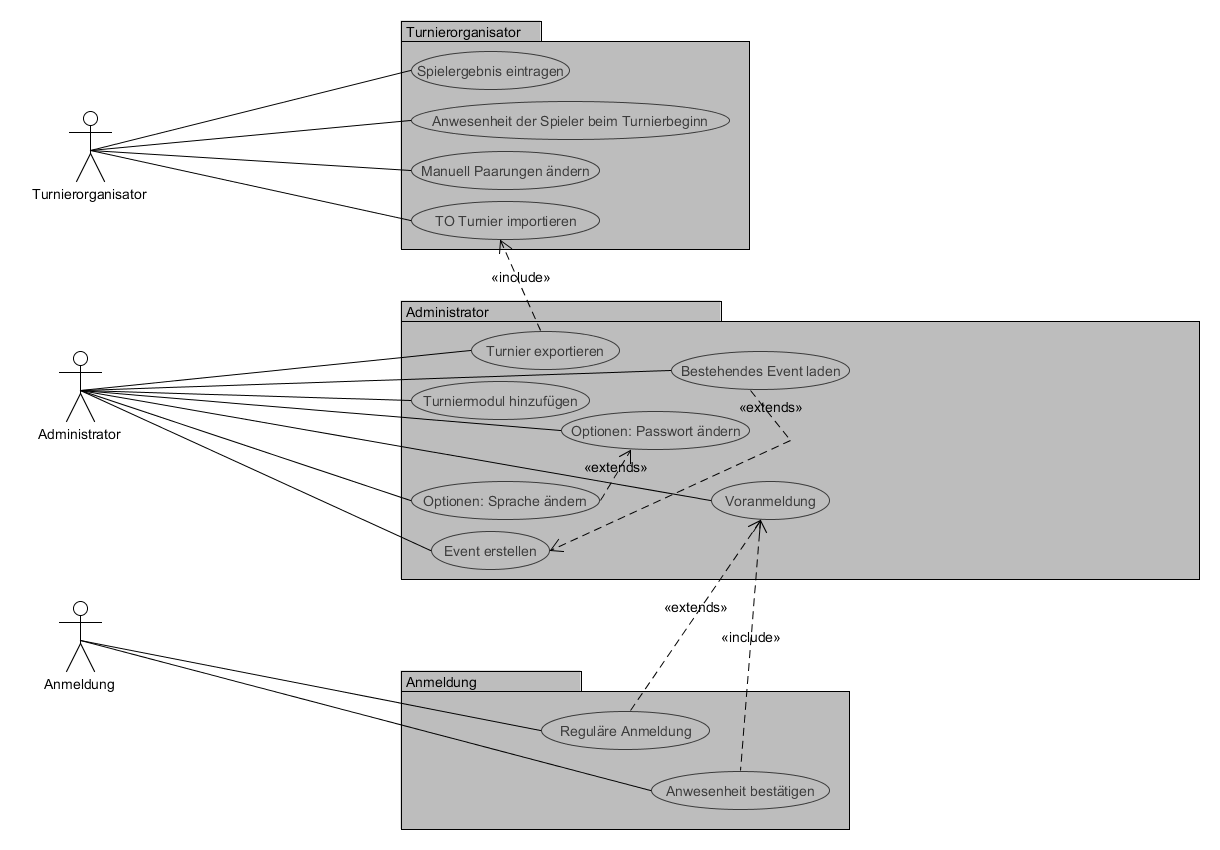
\includegraphics[width=\textwidth]{UseCaseDiagram.png}

\subsection{Anwendungsfälle des Administrators}

\subsubsection{Event erstellen}

\begin{tabularx}{\textwidth}{| p{0.2\textwidth} | p{0.7415\textwidth} |}
	\hline
	\textbf{Ziel} & Es kann mit der Voranmeldung begonnen werden, daher ist das Event mit allen notwendigen Daten fertig erstellt \\
	\hline
	\textbf{Akteure} & Administrator \\
	\hline
	\textbf{Beschreibung} & Es wird das Event erstellt und mit den vorhanden Daten modifiziert \\
	\hline
	\textbf{Ebene} & Benutzersicht \\
	\hline
	\textbf{Priorität} & Niedrig \\
	\hline
	\multicolumn{2}{| c |}{\textbf{Normalablauf}} \\
	\hline
	\textbf{Vorbedingung} & Anwendung wurde gestartet, Anwendung wurde falls nötig entsperrt \\
	\hline
	\textbf{Ablauf} &
		\begin{enumerate}
			\item[1.] Administrator: Nutzer startet das Erstellen des Events durch Drücken des Buttons "Event erstellen"
			\item[2.] System: Öffnet den Dialog für das Erstellen der Events
			\item[3.] Administrator: Nutzer vergibt Startdatum, Enddatum, Titel und öffnet das Fenster um die Turniere hinzuzufügen
			\newline
			Sonderfall für Alternativablauf 3a: Standard-Module sind nicht vorhanden
			\item[4.] System: Erstellt Datenbank für Vorabanmeldung
			\item[5.] System: Öffnet Dialog um Speicherort des Event zu bestimmen
			\item[6.] Administrator: Nutzer wählt den Speicherort aus
			\item[7.] System: Speichert das Event an dem vogegebenen Ort
			\newline
			Sonderfall für Alternativablauf 7a: Ungenügende Berechtigung um in den Zielordner zu schreiben
		\end{enumerate}
	\\
	\hline
	\textbf{Nachbedingung} & Vorabanmeldung kann gestartet werden, Event wurde gespeichert \\
	\hline
	\multicolumn{2}{| c |}{\textbf{Alternativablauf 3a}} \\
	\hline
	\textbf{Vorbedingung} & Standard-Module sind nicht vorhanden \\
	\hline
	\textbf{Ablauf} &
		\begin{enumerate}
			\item[3a1.] System: Gibt eine Meldung aus, dass die Standard-Module nicht gefunden wurden und verweist auf das Erstellen eines neuen Turniermoduls
			\item[3a2.] Administrator: Erstellt ein Turniermodul (siehe Use Case 5: Turniermodul erstellen)
			\newline
			Sonderfall für Alternativablauf 3a2a: Schließt Dialog ohne ein neues Turniermodul zu erstellen
			\item[3a3.] Administrator: Der Nutzer fügt dieses daraufhin dem Event hinzu
		\end{enumerate}
	\\
	\hline
	\textbf{Nachbedingung} & Das Event enthält nun ein oder mehrere Turniere \\
	\hline
	\multicolumn{2}{| c |}{\textbf{Alternativablauf 3a2a}} \\
	\hline
	\textbf{Vorbedingung} & Schließt Dialog ohne ein neues Turniermodul zu erstellen \\
	\hline
	\textbf{Ablauf} &
		\begin{enumerate}
			\item[3a2a1.] System: Geht in Zustand Y über
		\end{enumerate}
	\\
	\hline
	\textbf{Nachbedingung} & Zustand Y \\
	\hline
	\multicolumn{2}{| c |}{\textbf{Alternativablauf 7a}} \\
	\hline
	\textbf{Vorbedingung} & Ungenügende Berechtigung um in den Zielordner zu schreiben \\
	\hline
	\textbf{Ablauf} &
		\begin{enumerate}
			\item[7a1.] System: Gibt eine Warnung aus, dass eine ungenügende Schreibberechtigung vorhanden ist
		\end{enumerate}
	\\
	\hline
	\textbf{Nachbedingung} & Nutzer wurde infomiert, dass er ein neues Speicherziel wählen muss oder seine Änderungen werden nicht gespeichert \\
	\hline
\end{tabularx}

\subsection{Bestehendes Event laden}

\begin{tabularx}{\textwidth}{| p{0.2\textwidth} | p{0.7415\textwidth} |}
	\hline
	\textbf{Ziel} & Bestehendes Event aus dem gespeicherten Zustand laden \\
	\hline
	\textbf{Akteure} & Administrator \\
	\hline
	\textbf{Beschreibung} & Lädt das gespeicherte Event inklusive Turniermodulen, Zuständen und Fortschritt im Turnier Fragt gegebenenfalls ein gesetztes Passwort ab \\
	\hline
	\textbf{Ebene} & Benutzersicht \\
	\hline
	\textbf{Priorität} & Niedrig \\
	\hline
	\multicolumn{2}{| c |}{\textbf{Normalablauf}} \\
	\hline
	\textbf{Vorbedingung} & Programm ist gestartet, Anwendung ist entsperrt falls nötig \\
	\hline
	\textbf{Ablauf} &
		\begin{enumerate}
			\item[1.] Administrator: Drückt den 'Event laden'-Button
			\item[2.] System: Öffnet den File Browser
			\item[3.] Administrator: Wählt die zu ladende Datei aus der Verzeichnisstruktur aus und drückt laden
			\item[4.] System: Lädt den gespeicherten Zustand des Events
		\end{enumerate}
	\\
	\hline
	\textbf{Nachbedingung} & Der gespeicherte Zustand des Events ist geladen und benutzbar \\
	\hline
\end{tabularx}

\subsection{Optionen (Sprache anzeigen und ändern)}

\begin{tabularx}{\textwidth}{| p{0.2\textwidth} | p{0.7415\textwidth} |}
	\hline
	\textbf{Ziel} & Die aktuellen Optionen des Programms wie Sprache zu ändern oder anzuzeigen \\
	\hline
	\textbf{Akteure} & Administrator \\
	\hline
	\textbf{Beschreibung} &  \\
	\hline
	\textbf{Ebene} & Benutzersicht \\
	\hline
	\textbf{Priorität} & Niedrig \\
	\hline
	\multicolumn{2}{| c |}{\textbf{Normalablauf}} \\
	\hline
	\textbf{Vorbedingung} & Programm wurde gestartet \\
	\hline
	\textbf{Ablauf} &
		\begin{enumerate}
			\item[1.] Administrator: Öffnet die Optionen durch Betätigen des Optionen-Buttons
			\item[2.] System: Öffnet das Optionen-Fenster, zeigt aktuelle Spracheneinstellung an
			\item[3.] Administrator: Wählt andere Sprache aus
			\newline
			Sonderfall für Alternativablauf 3a: Will sich die Optionen nur anzeigen lassen und nicht verändern
			\newline
			Sonderfall für Alternativablauf 3b: Eingestellte Option ist dieselbe Sprache wie die aktuell ausgewählte
			\item[4.] System: Stellt die Sprache auf die ausgewählte Sprache um
		\end{enumerate}
	\\
	\hline
	\textbf{Nachbedingung} &  \\
	\hline
	\multicolumn{2}{| c |}{\textbf{Alternativablauf 3a}} \\
	\hline
	\textbf{Vorbedingung} & Will sich die Optionen nur anzeigen lassen und nicht verändern \\
	\hline
	\textbf{Ablauf} &
		\begin{enumerate}
			\item[3a1.] System: Es wird nichts verändert
			\item[3a2.] Administrator: Drückt den 'Zurück'-Button
		\end{enumerate}
	\\
	\hline
	\textbf{Nachbedingung} &  \\
	\hline
	\multicolumn{2}{| c |}{\textbf{Alternativablauf 3b}} \\
	\hline
	\textbf{Vorbedingung} & Eingestellte Option ist dieselbe Sprache wie die aktuell ausgewählte \\
	\hline
	\textbf{Ablauf} &
		\begin{enumerate}
			\item[3b1.] System: Belässt aktuelle Spracheinstellung
		\end{enumerate}
	\\
	\hline
	\textbf{Nachbedingung} & Programm wird in der eingestellten Sprache angezeigt \\
	\hline
\end{tabularx}

\subsection{Optionen (Passwort ändern)}

\begin{tabularx}{\textwidth}{| p{0.2\textwidth} | p{0.7415\textwidth} |}
	\hline
	\textbf{Ziel} & Es soll ein neues Passwort gesetzt werden oder ein bestehendes geändert werden \\
	\hline
	\textbf{Akteure} & Administrator \\
	\hline
	\textbf{Beschreibung} & Der Nutzer möchte seine Anwendung mit einem Passwort sichern oder das 
          bestehende Passwort ändern \\
	\hline
	\textbf{Ebene} & Benutzersicht \\
	\hline
	\textbf{Priorität} & Niedrig \\
	\hline
	\multicolumn{2}{| c |}{\textbf{Normalablauf}} \\
	\hline
	\textbf{Vorbedingung} & Anwendung ist gestartet, Anwendung ist falls nötig entsperrt \\
	\hline
	\textbf{Ablauf} &
		\begin{enumerate}
			\item[1.] Administrator: Nutzer drückt den 'Optionen'-Button
			\item[2.] System: Öffnet Optionen-Fenster
			\item[3.] Administrator: Nutzer drückt den 'Passwort ändern'-Button
			\item[4.] System: Öffnet Dialog, in dem die Passwortänderung vollzogen wird
			\newline
			Sonderfall für Alternativablauf 4a: Es wurde noch kein Passwort gesetzt
			\item[5.] Administrator: Gibt altes Passwort falls vorhanden und danach 2 Mal das neue Passwort ein
			\item[6.] System: Ändert das Passwort um die Anwendung zu sperren
			\newline
			Sonderfall für Alternativablauf 6a: Nutzer hat das 'Neues Passwort' Feld leer gelassen
		\end{enumerate}
	\\
	\hline
	\textbf{Nachbedingung} & Anwendung wird nach der Änderung mit dem neuen Passwort entsperrt \\
	\hline
	\multicolumn{2}{| c |}{\textbf{Alternativablauf 4a}} \\
	\hline
	\textbf{Vorbedingung} & Es wurde noch kein Passwort gesetzt \\
	\hline
	\textbf{Ablauf} &
		\begin{enumerate}
			\item[4a1.] System: Der Dialog enthält nur die Felder: 'Neues Passwort', 'Neues Passwort wiederholen';
		\end{enumerate}
	\\
	\hline
	\textbf{Nachbedingung} & Der Nutzer muss das nicht vorhandene Passwort nicht eingeben \\
	\hline
	\multicolumn{2}{| c |}{\textbf{Alternativablauf 6a}} \\
	\hline
	\textbf{Vorbedingung} & Nutzer hat das 'Neues Passwort' Feld leer gelassen \\
	\hline
	\textbf{Ablauf} &
		\begin{enumerate}
			\item[6a1.] System: Das Passwort wird entfernt
		\end{enumerate}
	\\
	\hline
	\textbf{Nachbedingung} & Nutzer kann Anwendung nicht mehr sperren \\
	\hline
\end{tabularx}

\subsection{Turniermodul hinzufügen}

\begin{tabularx}{\textwidth}{| p{0.2\textwidth} | p{0.7415\textwidth} |}
	\hline
	\textbf{Ziel} & Der Nutzer will eine Turniervariante erstellen \\
	\hline
	\textbf{Akteure} & Administrator \\
	\hline
	\textbf{Beschreibung} & Es wird ein neues Turniermodul erstellt, das weitgehend frei modifizierbar 
          ist und nachher als Vorlage für andere Events dienen kann \\
	\hline
	\textbf{Ebene} & Benutzersicht \\
	\hline
	\textbf{Priorität} & Niedrig \\
	\hline
	\multicolumn{2}{| c |}{\textbf{Normalablauf}} \\
	\hline
	\textbf{Vorbedingung} & Tourney ist geöffnet, Der Nutzer befindet sich auf der Startseite oder beim Erstellen eines Events in der Phase, in der die Turniere hinzugefügt werden \\
	\hline
	\textbf{Ablauf} &
		\begin{enumerate}
			\item[1.] Administrator: Nutzer drückt auf den 'Turniervorlage erstellen' Button
			\item[2.] System: Es öffnet sich ein Fenster, in dem der Nutzer die spezifischen Einstellungen für das Turnier vornehmen kann
			\item[3.] Administrator: Stellt die Einstellung ein und drückt daraufhin den 'Speichern'-Button
			\item[4.] System: Das Programm speichert die Einstellungen im Programmverzeichnis
			\newline
			Sonderfall für Alternativablauf 4a: Die Vorlage kann nicht gespeichert werden
		\end{enumerate}
	\\
	\hline
	\textbf{Nachbedingung} & Nutzer hat eine neue Vorlage für Turniere erstellt und kann diese in den Events verwenden \\
	\hline
	\multicolumn{2}{| c |}{\textbf{Alternativablauf 4a}} \\
	\hline
	\textbf{Vorbedingung} & Die Vorlage kann nicht gespeichert werden \\
	\hline
	\textbf{Ablauf} &
		\begin{enumerate}
			\item[4a1.] System: Zeigt eine Warnung an, dass die Änderungen nicht gespeichert werden können
		\end{enumerate}
	\\
	\hline
	\textbf{Nachbedingung} & Der Nutzer weiß, dass seine Änderung nicht gespeichert wurde \\
	\hline
\end{tabularx}

\subsection{Voranmeldung von Spielern}

\begin{tabularx}{\textwidth}{| p{0.2\textwidth} | p{0.7415\textwidth} |}
	\hline
	\textbf{Ziel} & Voranmeldungen vor dem Event erfassen und speichern \\
	\hline
	\textbf{Akteure} & Administrator \\
	\hline
	\textbf{Beschreibung} & Der Nutzer hat von mindestens einem Spieler Voranmeldungen erhalten und 
          möchte diese in das Event eintragen \\
	\hline
	\textbf{Ebene} & Benutzersicht \\
	\hline
	\textbf{Priorität} & Niedrig \\
	\hline
	\multicolumn{2}{| c |}{\textbf{Normalablauf}} \\
	\hline
	\textbf{Vorbedingung} & Anwendung wurde gestartet, Der Nutzer hat ein Event erstellt und befindet sich in der Phase Voranmeldung, Die Anwendung ist entsperrt, Der übermittelte Datensatz ist vollständig \\
	\hline
	\textbf{Ablauf} &
		\begin{enumerate}
			\item[1.] Administrator: Drückt den 'Spieler eintragen'-Button
			\item[2.] System: Öffnet die Maske um die Daten einzutragen
			\item[3.] Administrator: Trägt den Teilnehmer in die Maske ein (Name, Vorname, Turniere an denen er teilnehmen möchte, optional E-Mail-Adresse und Vorname)
			\item[4.] System: Überprüft, ob alle Angaben korrekt sind und trägt diese in die Datendank ein
			\newline
			Sonderfall für Alternativablauf 4a: Getätigte Eingabe ist inkorrekt
		\end{enumerate}
	\\
	\hline
	\textbf{Nachbedingung} & Teilnehmer ist in Datenbank eingetragen \\
	\hline
	\multicolumn{2}{| c |}{\textbf{Alternativablauf 4a}} \\
	\hline
	\textbf{Vorbedingung} & Getätigte Eingabe ist inkorrekt \\
	\hline
	\textbf{Ablauf} &
		\begin{enumerate}
			\item[4a1.] System: Gibt eine Fehlermeldung aus und lässt Nutzer die Eingaben nochmal überprüfen und verändern
		\end{enumerate}
	\\
	\hline
	\textbf{Nachbedingung} & Eingabe ist korrekt \\
	\hline
\end{tabularx}

\subsection{Reguläre Anmeldung eines Spielers}

\begin{tabularx}{\textwidth}{| p{0.2\textwidth} | p{0.7415\textwidth} |}
	\hline
	\textbf{Ziel} & Der Spieler soll in die Datenbank eingetragen sein und für die einzelnen 
          Turniere registriert sein \\
	\hline
	\textbf{Akteure} & Anmeldung, Spieler \\
	\hline
	\textbf{Beschreibung} & Spieler meldet sich bei der Anmeldung für verschiedene Turniere an. Dies 
          wird dann in die Datenbank geschrieben \\
	\hline
	\textbf{Ebene} & Benutzersicht \\
	\hline
	\textbf{Priorität} & Niedrig \\
	\hline
	\multicolumn{2}{| c |}{\textbf{Normalablauf}} \\
	\hline
	\textbf{Vorbedingung} & Anwendung wurde gestartet, Der Administrator hat ein Event erstellt, Die Anmeldung hat dieses Event importiert, Anwendung ist entsperrt, Das Event befindet sich in der Phase Anmeldung \\
	\hline
	\textbf{Ablauf} &
		\begin{enumerate}
			\item[1.] Spieler: Gibt der Anmeldung die erforderlichen Daten zum Anmelden
			\item[2.] Anmeldung: Gibt Daten in dafür vorgesehene Maske ein
			\item[3.] System: Trägt die Daten in die Datenbank ein
		\end{enumerate}
	\\
	\hline
	\textbf{Nachbedingung} & Spieler befindet sich in der Event-Datenbank \\
	\hline
\end{tabularx}

\subsection{Anwesenheit eines vorangemeldeten Spielers bestätigen}

\begin{tabularx}{\textwidth}{| p{0.2\textwidth} | p{0.7415\textwidth} |}
	\hline
	\textbf{Ziel} & Die Anwesenheit der vorangemeldeten Spieler zu bestätigen und die 
          Bezahlung der Gebühr abzuwickeln \\
	\hline
	\textbf{Akteure} & Spieler, Anmeldung \\
	\hline
	\textbf{Beschreibung} & Der vorangemeldete Spieler gibt seinen Namen/E-Mail-Adresse der Anmeldung. Diese 
          sucht daraufhin in der Datenbank nach dem Namen und bestätigt, dass 
          dieser anwesend ist und bezahlt hat \\
	\hline
	\textbf{Ebene} & Benutzersicht \\
	\hline
	\textbf{Priorität} & Niedrig \\
	\hline
	\multicolumn{2}{| c |}{\textbf{Normalablauf}} \\
	\hline
	\textbf{Vorbedingung} & Anwendung muss gestartet sein, Anwendung muss entsperrt sein, Das Event muss erstellt worden sein, Das Event muss sich in der Phase 'Anmeldung' befinden, Das Event muss von der Anmeldung importiert worden sein, Spieler muss in der Datenbank enthalten sein \\
	\hline
	\textbf{Ablauf} &
		\begin{enumerate}
			\item[1.] Spieler: Gibt der Anmeldung Name/E-Mail-Adresse
			\item[2.] Anmeldung: Drückt den 'Voranmeldung verifizieren'-Button
			\item[3.] System: Öffnet die Maske, in der Name und E-Mail-Adresse eingegeben werden
			\item[4.] Anmeldung: Gibt Name und E-Mail-Adresse ein und setzt Haken (Anwesenheit, bezahlt) und betätigt 'Verifizieren'-Button
			\item[5.] System: Ändert Datenbankeintrag des Spielers und fügt ihn dem Turnier/den Turnieren hinzu
		\end{enumerate}
	\\
	\hline
	\textbf{Nachbedingung} & Spieler ist verifiziert und den Turnieren hinzugefügt \\
	\hline
\end{tabularx}

\subsection{Turnier exportieren}

\begin{tabularx}{\textwidth}{| p{0.2\textwidth} | p{0.7415\textwidth} |}
	\hline
	\textbf{Ziel} & Turnier ist als Datei exportiert \\
	\hline
	\textbf{Akteure} & Administrator \\
	\hline
	\textbf{Beschreibung} & Das Turnier soll an den Turnierorganisator weitergegeben werden, 
          dieser kann das einzelne Turnier importieren \\
	\hline
	\textbf{Ebene} & Benutzersicht \\
	\hline
	\textbf{Priorität} & Niedrig \\
	\hline
	\multicolumn{2}{| c |}{\textbf{Normalablauf}} \\
	\hline
	\textbf{Vorbedingung} & Anwendung muss gestartet sein, Anwendung muss entsperrt sein, Ein Event muss erstellt sein, Das Event muss in der Phase 'Turniere exportieren' sein \\
	\hline
	\textbf{Ablauf} &
		\begin{enumerate}
			\item[1.] Administrator: Drückt den Button 'Turnier exportieren'
			\item[2.] System: Öffnet das Fenster zum Auswählen des Speicherorts für das exportierte Turnier
			\item[3.] Administrator: Exportiert das Turnier
		\end{enumerate}
	\\
	\hline
	\textbf{Nachbedingung} & Turnier muss exportiert sein \\
	\hline
\end{tabularx}

\subsection{Turnier durch Turnierordner importieren}

\begin{tabularx}{\textwidth}{| p{0.2\textwidth} | p{0.7415\textwidth} |}
	\hline
	\textbf{Ziel} & Das Turnier soll importiert sein \\
	\hline
	\textbf{Akteure} & Turnierordner \\
	\hline
	\textbf{Beschreibung} & Der Turnierordner bekommt die Datei des Turniers und importiert dieses \\
	\hline
	\textbf{Ebene} & Benutzersicht \\
	\hline
	\textbf{Priorität} & Niedrig \\
	\hline
	\multicolumn{2}{| c |}{\textbf{Normalablauf}} \\
	\hline
	\textbf{Vorbedingung} & Die Anwendung muss gestartet sein, Die Anwendung muss entsperrt sein, Das exportierte Turniermodul muss vorhanden sein, Nutzer muss auf der Startseite sein \\
	\hline
	\textbf{Ablauf} &
		\begin{enumerate}
			\item[1.] Turnierordner: Drückt den Button 'Turnier importieren'
			\item[2.] System: Öffnet den File Browser um das Turnier zu importieren
			\item[3.] Turnierordner: Wählt die exportierte Turnier-Datei aus
			\item[4.] System: Importiert das Turnier
		\end{enumerate}
	\\
	\hline
	\textbf{Nachbedingung} & Das Turnier muss importiert sein \\
	\hline
\end{tabularx}

\subsection{Anwesenheit der Spieler bei Turnierbeginn}

\begin{tabularx}{\textwidth}{| p{0.2\textwidth} | p{0.7415\textwidth} |}
	\hline
	\textbf{Ziel} & Anwesenheit der Spieler beim Turnierbeginn feststellen \\
	\hline
	\textbf{Akteure} & Turnierordner \\
	\hline
	\textbf{Beschreibung} & Der Turnierordner überprüft die Anwesenheit der einzelnen Spieler, damit 
          die Paarungen bestimmt werden können \\
	\hline
	\textbf{Ebene} & Benutzersicht \\
	\hline
	\textbf{Priorität} & Niedrig \\
	\hline
	\multicolumn{2}{| c |}{\textbf{Normalablauf}} \\
	\hline
	\textbf{Vorbedingung} & Anwendung muss gestartet sein, Anwendung muss entsperrt sein, Turnier muss geladen sein, Turnier mus in der Phase 'Anwesenheit kontrollieren' sein \\
	\hline
	\textbf{Ablauf} &
		\begin{enumerate}
			\item[1.] System: Zeigt eine Liste von Spielern an, die an diesem Turnier teilnehmen
			\item[2.] Turnierordner: Verifiziert die Anwesenheit der einzelnen Spieler
			\item[3.] System: Löscht jeden nicht verifizierten Spieler mit einer Warnung
		\end{enumerate}
	\\
	\hline
	\textbf{Nachbedingung} & Nur verifizierte Spieler befinden sich in der Turnier-Datenbank \\
	\hline
\end{tabularx}

\subsection{Spielergebnis eintragen}

\begin{tabularx}{\textwidth}{| p{0.2\textwidth} | p{0.7415\textwidth} |}
	\hline
	\textbf{Ziel} & Das Ergebnis einer Paarung eintragen \\
	\hline
	\textbf{Akteure} & Turnierordner \\
	\hline
	\textbf{Beschreibung} & Der Turnierordner trägt bei einer Paarung die Punktzahl und gegebenenfalls Sekundär/ 
          Tertiärwertungen ein \\
	\hline
	\textbf{Ebene} & Benutzersicht \\
	\hline
	\textbf{Priorität} & Niedrig \\
	\hline
	\multicolumn{2}{| c |}{\textbf{Normalablauf}} \\
	\hline
	\textbf{Vorbedingung} & Die Anwendung ist gestartet, Die Anwengung ist entsperrt, Das Turnier muss in einer laufenden Runde sein, Das Turnier muss importiert sein \\
	\hline
	\textbf{Ablauf} &
		\begin{enumerate}
			\item[1.] Turnierordner: Der Nutzer wählt die Paarung aus, die er bewerten will
			\item[2.] System: Zeigt die voreingestellten Ausgangsmöglichkeiten an
			\item[3.] Turnierordner: Nutzer wählt eine davon aus oder gibt die Wertungen manuell ein
		\end{enumerate}
	\\
	\hline
	\textbf{Nachbedingung} & Paarung muss bewertet sein \\
	\hline
\end{tabularx}

\subsection{Manuell Paarungen ändern}

\begin{tabularx}{\textwidth}{| p{0.2\textwidth} | p{0.7415\textwidth} |}
	\hline
	\textbf{Ziel} & Computergenerierte Paarungen ist von Hand geändert \\
	\hline
	\textbf{Akteure} & Turnierordner \\
	\hline
	\textbf{Beschreibung} & Der Turnierordner kann die computergenerierten Paarungen auch von Hand ändern \\
	\hline
	\textbf{Ebene} & Benutzersicht \\
	\hline
	\textbf{Priorität} & Niedrig \\
	\hline
	\multicolumn{2}{| c |}{\textbf{Normalablauf}} \\
	\hline
	\textbf{Vorbedingung} & Die Anwendung muss aktiv sein, Die Anwendung muss entsperrt sein, Das Turnier muss vor einer Runde sein, es darf noch keine Wertung eingetragen sein \\
	\hline
	\textbf{Ablauf} &
		\begin{enumerate}
			\item[1.] Turnierordner: Turnierordner wählt die zwei zu tauschenden Spieler aus und betätigt den 'Tauschen'-Button
			\item[2.] System: Tauscht die ausgewählten Spieler
		\end{enumerate}
	\\
	\hline
	\textbf{Nachbedingung} & Die getauschten Paarungen sollen gespeichert werden \\
	\hline
\end{tabularx}

\subsection{Anwendungsfälle der Turnierordner}

\section{Anhang}

\subsection{Begriffslexikon}

\subsection{Versionshistorie}

\begin{itemize}
	\item Version 1.0 (05.11.2014)
	\begin{itemize}
		\item Grundstruktur der Spezifikation erstellt
	\end{itemize}
	\item Version 1.1 (10.11.2014)
	\begin{itemize}
		\item Kapitel 1 und 2 hinzugefügt
	\end{itemize}
	\item Version 1.2 (11.11.2014)
	\begin{itemize}	
		\item Kapitel 4 hinzugefügt
	\end{itemize}
	\item Version 1.3 (12.11.2014)
	\begin{itemize}
		\item Kapitel 3.2 hinzugefügt
	\end{itemize}
\end{itemize}

\end{document}
